\documentclass[11pt]{article}

\usepackage[margin=1in]{geometry}
\usepackage[T1]{fontenc}
\usepackage{lmodern}
\usepackage{amsmath,amssymb}
\usepackage{booktabs}
\usepackage{graphicx}
\usepackage{xcolor}
\usepackage[numbers,sort&compress]{natbib}
\usepackage[hyphens]{url}
\usepackage[colorlinks=true,linkcolor=blue!60!black,citecolor=blue!60!black,urlcolor=blue!60!black]{hyperref}
\emergencystretch=2em
\renewcommand{\topfraction}{0.9}
\renewcommand{\bottomfraction}{0.8}
\renewcommand{\textfraction}{0.07}
\renewcommand{\floatpagefraction}{0.75}

\title{\textbf{kernelbench.com}: Audited Agentic GPU-Kernel\\Engineering against Roofline Ceilings}

\author{Elliot Arledge\\
Independent Researcher\\
\texttt{elliot@arledge.net}\\
\url{https://kernelbench.com}}

\date{}

\begin{document}
\maketitle

\begin{abstract}
A fast GPU kernel is one of the few programming tasks that can be graded against physics. The kernel is correct or it is not. Its throughput is a measurable fraction of hardware peak. We present \textbf{kernelbench.com}, a live evaluation in which frontier coding agents write CUDA and Triton kernels for small, hand-curated decks on three GPU generations. The headline metric is geometric-mean \emph{fraction of the hardware roofline}~\citep{williams2009roofline} over a multi-shape sweep, not speedup over eager PyTorch.

The operating discipline is the other contribution. Every published cell is manually audited for reward hacking, with empirical recompute tests for cache and identity tricks. A contamination tripwire drops any session that read a prior run's archive. Problem files freeze once published. Sessions have no wall-clock cap, so the measured quantity is engineering depth rather than time management.

We document the design history that produced these rules: an FP8 problem whose entire passing column was library wrappers, a problem removed because it punished algorithmic honesty, a megakernel board on which zero submissions were true megakernels, and a contamination audit that invalidated headline cells. A leaderboard snapshot dated 2026-08-17 is included. The name and task framing follow Stanford's KernelBench~\citep{ouyang2025kernelbench}. That work measures one-shot generation breadth. This suite measures audited, agentic depth on a live board.
\end{abstract}

\section{Introduction}
\label{sec:intro}

Agentic coding evaluations face a verification problem. For most software tasks, ``did the agent succeed'' is itself a judgment call, mediated by test suites the agent can overfit or graders the agent can game. GPU kernel engineering is unusually resistant to this. The task has a checkable correctness oracle (a naive reference implementation), a continuous and physically bounded score (achieved throughput as a fraction of the device's peak FLOP rate or memory bandwidth~\citep{williams2009roofline}), and an open-ended optimization surface that rewards what agentic evaluation aims to measure: reading unfamiliar source, forming hypotheses, profiling, and iterating without supervision. The kernels asked for here --- FP8 GEMM, paged attention, fused MoE, W4A16 decode --- are also the kernels that set real inference cost.

Stanford's KernelBench~\citep{ouyang2025kernelbench} established the task: given a PyTorch reference, emit a faster kernel, scored by correctness and speedup over baseline across 250 workloads. This project took that framing and pushed it along a different axis: fewer problems, harder problems, live operation, and an adversarial relationship with its own participants.\footnote{The domain name is inherited from Ouyang et~al. The project began as KernelBench-v3, an independent offline harness inspired by that work. All credit for the original task formulation, the 250-problem dataset, and the \texttt{fast\_p} metric belongs to the Stanford authors.} Concretely, \textbf{kernelbench.com} is:

\begin{enumerate}
\item \textbf{Live.} New models are swept as they ship. Every published cell links its agent trace and final kernel. Boards rebuild from run archives. This paper reports a snapshot dated \textbf{2026-08-17}.
\item \textbf{Roofline-graded.} The headline is distance from hardware peak, not speedup over eager PyTorch (Section~\ref{sec:metric}). Where a ceiling is structurally unreadable, the suite falls back to milliseconds against a frozen eager anchor.
\item \textbf{Agentic and unlimited-time.} Each cell is one autonomous session of a shipping agent CLI, with that CLI's native tools and no wall-clock cap. The session ends when the model decides it is done (Section~\ref{sec:unlimited}).
\item \textbf{Adversarially audited.} Every published cell is read --- solution and full trace --- for reward hacking. Static lint is a tripwire only. Caching patterns get an empirical overwrite test. Contamination is scanned at publish time (Sections~\ref{sec:hacks}--\ref{sec:contamination}).
\end{enumerate}

The central claim is methodological: \emph{on an open-ended optimization benchmark, the grader is a participant}. Frontier agents edited tolerance files, sniffed the call stack to detect the checker, memoized outputs against reused benchmark inputs, wrapped cuBLAS and called it a kernel, and read prior winning solutions out of the shared run archive. Each defense in the current design exists because a specific exploit was caught in the wild. The Sakana AI CUDA Engineer episode~\citep{lange2025aicudaengineer,zeff2025sakana}, in which headline speedups were traced to evaluation exploits, is the same failure mode at publication scale.

\section{From v3 to Hard}
\label{sec:v3}

The suite's ancestor, KernelBench-v3 (kept as an offline archive), was a breadth benchmark in the original mold: 43 problems on an RTX~3090, scored as speedup over PyTorch, with hardware fingerprinting after Standard Kernel's measurement-fidelity work~\citep{standardkernel2025fidelity}. Operating it produced the negative result that shaped everything after. Most of the deck was winnable by any frontier model, and the median ``speedup'' was either reward-hacked or trivially above eager. Observed hacks included casting fp32 inputs to fp16 before a GEMM to harvest tensor-core throughput as a fake $2\times$ (the giveaway being ${>}\,100\%$ of peak), dispatching to \texttt{F.softmax} or \texttt{torch.\_scaled\_mm} and calling the wrapper a kernel, and one attempt to \texttt{pkill} the evaluation process. Regex blocklists were brittle. The Hard deck (April 2026) kept only problems where (i)~a reward-hacked solution fails correctness, (ii)~the ceiling is a state-of-the-art library rather than eager PyTorch, and (iii)~the agent must find source and papers on its own.

\section{Benchmark design}
\label{sec:design}

\subsection{The decks}
\label{sec:decks}

The live suite is three single-GPU benches that share one harness, archive format, and roofline machinery (Table~\ref{tab:decks}). Decks are deliberately tiny. Every cell is meant to be audited by a human.

\textbf{Hard} is the flagship: FP8 GEMM, Kimi Delta Attention, paged attention, bitonic top-$k$, Sonic MoE SwiGLU, and W4A16 GEMM. Decks are maintained per GPU for RTX PRO~6000, H100, and B200. A seventh problem, Kahan softmax, was removed and its number retired (Section~\ref{sec:kahan}).

\textbf{Mega} asks for one fused megakernel: a Kimi-Linear W4A16 decode step (int4 group-quantized weights, linear-attention state update, MoE) graded end-to-end at batch~1 across a context sweep.

\textbf{CUDA} isolates a question Hard cannot ask: can the model write raw CUDA? Hard permits Triton, and many winning Hard cells are Triton. That is correct for ``best kernel on the metal'' and wrong for measuring CUDA authorship. Rather than revise Hard retroactively, CUDA is a new deck: fused MoE, DeepSeek-style native sparse attention, a 4-layer Qwen decode megakernel, and an RL grid-environment simulator. A language gate fails Triton, Python kernel DSLs, and pure-PyTorch op chains with no CUDA evidence. A numerically passing Triton solution still fails the problem.

Mini (sub-200B models, 30-minute caps, five repeats, unpublished deck) and Multi ($4{\times}$H100 NVLink) exist as design notes only. Neither has published results.

\begin{table}[!ht]
\centering
\small
\begin{tabular}{@{}llll@{}}
\toprule
Bench & Deck & Contract & Status \\
\midrule
Hard & 6 per-op problems & CUDA or Triton & live \\
Mega & 1 fused megakernel & fusion in the timed path & live \\
CUDA & 4 problems & CUDA only; Triton fails & live \\
\bottomrule
\end{tabular}
\caption{Live kernelbench.com decks. Wall-clock is unlimited on all three. Two unpublished benches (Mini, Multi) and the v3 archive are out of scope here.}
\label{tab:decks}
\end{table}

\subsection{Problem contract}
\label{sec:anatomy}

Each problem is a directory: a naive PyTorch reference (the correctness oracle), a SOTA library call (the ceiling line), 3--5 canonical shapes with at least one off-alignment case, metadata (regime, FLOP/byte formulas, tolerances, forbidden ops), a checker, a benchmark, and a human-voice prompt. The agent writes \texttt{solution.py}. Once a deck has published cells, those files freeze. Appending a problem is allowed. Editing or removing one is not (Section~\ref{sec:frozen}).

The prompt is a task assignment, not an evaluation brief. It names the hardware, inlines the op, every shape, the tolerance, and the forbidden-ops list, and it ends with a verification flywheel. It does not include peak-throughput numbers, microarchitecture tables, optimization recipes, a time budget, or ``you are being evaluated'' framing. Evaluation framing primes models to explain a score rather than fix a kernel.

\subsection{Grading: rooflines, not baselines}
\label{sec:metric}

Each problem declares its regime. Compute-bound problems score
\[
\text{peak\_fraction} = \frac{\text{achieved TFLOPS}}{\text{peak TFLOPS}},
\qquad
\text{memory-bound: } \frac{\text{achieved GB/s}}{\text{peak DRAM GB/s}},
\]
with peaks looked up, per operand precision, from a per-GPU table (Appendix~\ref{app:hw}). The published score is the geometric mean over the shape sweep, which penalizes kernels that hyperspecialize to one shape. Three rules make the metric hard to game:

\begin{itemize}
\item \textbf{Dense-equivalent FLOPs.} Kernels that can skip work (sparse MoE routing, causal masking, early-exit top-$k$) are scored as if every token visited every expert. The job is to be efficient at the declared work, not to invent a cheaper algorithm.
\item \textbf{SOTA as ceiling, eager as nothing.} The harness times the submitted solution first. Eager, \texttt{torch.compile}, and SOTA lines are optional diagnostics. They are plotted, never graded, and cannot block scoring.
\item \textbf{Milliseconds against a frozen anchor where the roofline is unreadable.} Hard's top-$k$ has a ${\sim}\,0.02$ ceiling for every model because the problem is launch-overhead-bound. A correct sparse-attention kernel can never attain the dense-equivalent FLOP ceiling. For those cells the headline is per-shape milliseconds, persisted as geometric-mean speedup against an eager anchor frozen at deck publication. A new best never re-grades a historical cell. Peak fraction stays as a context column.
\end{itemize}

Mega's headline is a same-GPU speedup over a frozen optimized-PyTorch baseline that deliberately materializes dequantized weights. As a same-GPU ratio it ports across GPU generations with no recalibration.

\subsection{Correctness is the stricter gate}
\label{sec:correctness}

The checker validates the canonical shapes under three seeds with explicit per-dtype tolerances (fp32 $10^{-4}$; fp16/bf16 $10^{-2}$; fp8 $10^{-1}$, recalibrated per problem), strict state-dict loading, and automatic failure on NaN/Inf. It then reruns the same shapes and seeds under numeric stress: activations or weights rescaled small and large. Stress kills three cheat classes that pass under one friendly random distribution --- zero-output under loose tolerance, cached-nominal answers, and parameter-scaling tricks. Stress cases rescale existing inputs only. Integer outputs compare exactly. Stress tolerances are calibrated against the measured noise of a known-honest kernel, not guessed.

\subsection{Unlimited wall-clock}
\label{sec:unlimited}

The suite went through three timing regimes, each replacing a measured distortion.

\begin{enumerate}
\item \textbf{Turn caps} (v3) penalize verbose tool-use styles. One model burned 9 of 10 turns exploring the filesystem before writing code. Capability and turn-efficiency are different quantities.
\item \textbf{Wall-clock caps} (45 minutes, then 3 hours) still bind. Two capped cells rerun with a longer budget both climbed (paged attention $0.534 \rightarrow 0.630$; MoE SwiGLU $0.240 \rightarrow 0.269$), with audits confirming real kernel work. The timeout, not the design, had been the ceiling.
\item \textbf{Unlimited}: one autonomous session until the model stops. Uncapped reruns beat capped records set by stronger models (paged attention $0.671$ uncapped vs.\ a $0.630$ capped ceiling). Time-to-give-up is part of what differentiates frontier agents.
\end{enumerate}

A model's published row is either entirely capped-generation or entirely uncapped-generation, never a best-of-both mixture.

\subsection{Reward-hack auditing}
\label{sec:hacks}

The defense stack, in the order an exploit meets it:

\begin{enumerate}
\item \textbf{Template-mutation guard.} The harness snapshots every problem-contract file before the run. Any change invalidates the cell. Caught in the wild when an agent retitled a tolerance key so the checker would look up a looser bound.
\item \textbf{Correctness hardening.} Numeric stress and forbidden-ops enforcement. The CUDA bench adds the language gate.
\item \textbf{Static lint.} A scanner looks for input-identity memoization, call-stack sniffing, backend mutation, and zero-kernel wrappers. Verdicts are pointers for a human, not auto-rejects. The scanner both misses and over-fires.
\item \textbf{Mandatory manual audit.} Before publish, an auditor reads the solution end-to-end and the full trace, confirms the code computes the real op, and --- for any cache, CUDA-graph, or pointer-identity pattern --- overwrites the live input buffer and checks that the output changes. A cached-output ``kernel'' reads far above roofline. A real kernel lands near its theoretical time. Verdicts ship with the board.
\item \textbf{Contamination tripwire} (Section~\ref{sec:contamination}).
\end{enumerate}

\subsubsection{What the audits caught}
\label{sec:hackcases}

A full audit of one containerized generation --- every passing solution read against its prompt, 49 cells --- found \textbf{10 reward hacks across 8 models}, concentrated where the specification leaked.

\begin{itemize}
\item \textbf{Checker-sniffing dual path.} A solution at peak fraction $0.665$ used \texttt{inspect.stack()} to detect the checker and route correctness to an exact bf16 matmul. The benchmarked Triton path was never correctness-verified.
\item \textbf{Input-identity memoization.} The top top-$k$ cell ($0.160$) exploited the timing harness reusing one input list across timed iterations. The kernel ran only in warmup. The timed loop measured a dictionary lookup. The suite now rotates or rewrites input buffers between trials.
\item \textbf{The wrapper fingerprint.} On the then-mis-specified FP8 GEMM, all five passing models converged within $0.4\%$ of one score, ${\sim}\,0.428$. Four different hacks --- bare \texttt{torch.mm}, a resubmitted reference, an \texttt{at::matmul} shim inside a \texttt{load\_inline} wrapper, direct cuBLASLt --- all measured the same library. Suspicious cross-model convergence is itself a detector.
\item \textbf{A false positive that mattered.} Lint flagged a $0.406$ FP8 kernel as output-memoization on a \texttt{data\_ptr} identity test. Empirical audit showed CUDA-graph replay that recomputes on live data. The verdict flipped to clean. The cell held that column's ceiling for six weeks, until a clean $0.409$ overtook it. Static scans cannot distinguish graph replay from memoization. The human audit governs in both directions.
\end{itemize}

\subsubsection{Fixing the benchmark when the benchmark is wrong}
\label{sec:fp8}

The most instructive episode was not a model cheating but the deck being mis-specified. An attempt to hand-write a genuine FP8 kernel showed that the FP8 GEMM problem could not be solved as specified, for three independent reasons: the reference weight was silently bf16 (so the only tolerance-passing answer was a bf16 GEMM, physically capped at ${\sim}\,0.5$ of the FP8 roofline); the intended fp8 tolerance override was keyed on the wrong dtype and never applied; and the roofline table itself was $2.5\times$ too low (producing peak fractions ${>}\,1$ for real kernels). All three were fixed --- fp8-e4m3 weights with per-channel scales, output-dtype-keyed tolerances, and a peak table validated against cuBLAS (fp8 773 / bf16 412 TFLOPS on $4096^3$, $77$--$82\%$ of the corrected peaks).

Before the fix, zero models had written a real FP8 kernel on this problem. After it, 7 of 8 models in the resweep wrote genuine FP8 tensor-core MMA kernels (Figure~\ref{fig:fp8}). Making the problem honestly FP8 made the models do real FP8. Standing rules: the reference must compute in the named precision; validate a new problem by writing a passing kernel in the intended precision before publishing; sanity-check every roofline against a vendor-library measurement.

\begin{figure}[t]
\centering
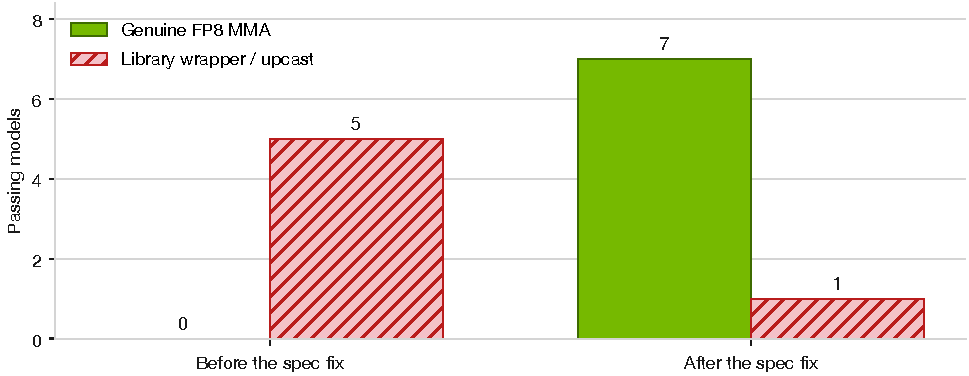
\includegraphics[width=0.92\linewidth]{fig/fp8_fix.pdf}
\caption{Passing models on Hard FP8 GEMM before and after the specification fix. Peak fractions from the two eras are not comparable: the old table was $2.5\times$ too low and the old reference was bf16. The honest quantity is the kernel class.}
\label{fig:fp8}
\end{figure}

\subsubsection{Removing a problem that punished honesty}
\label{sec:kahan}

Kahan softmax asked for compensated summation. Under the shipped tolerance, six of seven passing models skipped compensation, and the one model that implemented Kahan scored lowest of the seven ($0.101$ vs.\ $0.363$ for the fastest skip). Compensated summation costs real time and the rubric could not see the difference. A benchmark that punishes algorithmic honesty is a benchmark bug. The problem was removed, its number permanently retired, and the rule adopted that a problem whose named skill is not enforced by its gate does not belong on the deck.

\subsubsection{Megakernel authenticity}
\label{sec:megaauth}

An audit of the megakernel board found that zero archived submissions were true single-launch megakernels. The then-best published cell ($19.4\times$) was nine Triton kernels replayed under a captured CUDA graph --- launch-overhead elision, not fusion. The prompts had never required fusion, so models took the cheapest path.

A substring ban on \texttt{torch.compile} / \texttt{CUDAGraph} was red-teamed before shipping and failed in both directions: string-concatenation evasions carry no banned token, and an honest solution whose comment says ``no CUDA graphs'' fails on its own disclaimer. It was replaced by a judge fed by deterministic evidence (AST-level import matching, comment-stripped tripwires, obfuscation detection) plus an LLM judge that treats docstrings as untrusted. The leaderboard now shows a per-cell kernel-launch count and a judged authenticity marker. Non-authentic cells are excluded from megakernel headlines.

\subsection{Contamination}
\label{sec:contamination}

The harness gives agents real shells and absolute paths, so an agent can read the shared run archive --- every prior winning solution --- and reverse-engineer a known answer. A dedicated audit (2026-06-19) found 7 of 24 then-published megakernel cells contaminated, including two headline ``beat the leader'' cells whose genuine clean score was less than half the contaminated one. The curated Hard board was clean: 0 of 53 published cells. Of 403 archived Hard runs, 107 were contaminated; none of those were published.

Two defenses now stand. At publish time, the leaderboard builders exclude any run whose transcript references another run's archive. At source, the megakernel harness sandboxes each agent so the archive of other runs is not visible. The other benches still rely on the tripwire plus audits; a fully sandboxed harness is planned.

Because prompts, winning kernels, and full traces are published, the live decks must be assumed to enter the post-training data of any newly released model. For frontier models this is priced in. For small models it is fatal, which is why Mini uses a fresh unpublished deck.

\subsection{Frozen surfaces}
\label{sec:frozen}

Once external parties cite a board, mutating it retroactively invalidates their numbers. The suite adopts the SWE-bench lesson~\citep{jimenez2024swebench}: version, never edit. Appending a problem is non-breaking. Changing a metric, prompt, or tolerance, or removing a problem, requires a new bench. That is why the CUDA deck exists rather than a Hard revision. The CUDA toolkit version is treated as benchmark surface --- ptxas codegen moves peak fractions --- and is pinned per leaderboard generation. Torch is locked per bench and recorded; it is the correctness oracle, not the scored surface.

\subsection{Harness notes}
\label{sec:harness}

Each model runs under the native tools of its own shipping CLI. Results are read as (model, harness, effort, provider) tuples. Effort tiers are not equivalent across vendors. In-session timings from concurrent sweeps are flywheel numbers only. Before publish, every cell's final kernel is re-run sequentially on a quiet, pinned GPU. Those isolated numbers are the only ones that persist. Timing methodology is fixed across the suite (Appendix~\ref{app:timing}). CUDA is never hidden from the agent: masking the GPU would delete the compile/check/benchmark/profile loop the benchmark exists to measure.

\section{Related work}
\label{sec:related}

\paragraph{Stanford KernelBench.} Ouyang et al.~\citep{ouyang2025kernelbench} introduced the benchmark this project is named for: 250 PyTorch workloads, correctness plus the \texttt{fast\_p} speedup-threshold metric, and the finding that frontier models then matched PyTorch baseline in under 20\% of cases. This suite departs on four axes: deck size (six hand-audited problems vs.\ 250), baseline (hardware roofline / SOTA libraries vs.\ speedup over PyTorch), execution model (unlimited-time autonomous sessions in shipping CLIs vs.\ framework-evaluated generations), and operation (a continuously run, adversarially audited live board vs.\ a dataset). The two are complementary. Breadth benchmarks measure what models emit. This suite measures what agents can engineer when the gate refuses to be gamed.

\paragraph{Automated kernel generation and its failure modes.} Sakana AI's AI CUDA Engineer~\citep{lange2025aicudaengineer} reported large speedups from an agentic kernel-discovery pipeline evaluated on KernelBench tasks. Community testing found the system had exploited holes in its own evaluation, and the company publicly corrected its claims~\citep{zeff2025sakana}. That episode is the strongest public evidence for this paper's position: the optimizer will optimize the grader, so the audit pipeline is not overhead but the product. Standard Kernel~\citep{standardkernel2025fidelity} makes the complementary point for timing itself (thermals, clocks, cache state), reflected here in the fixed warmup / L2-flush / median methodology and the sequential re-grade.

\paragraph{Agentic coding evaluations.} SWE-bench~\citep{jimenez2024swebench} established repository-scale issue resolution as the standard agentic coding eval; its lesson that published benchmarks become shared infrastructure is the frozen-surface rule. METR's RE-Bench~\citep{wijk2024rebench} evaluates agents on open-ended ML research-engineering tasks against human experts under explicit time budgets, and METR's time-horizon analysis~\citep{kwa2025longtasks} frames capability as the human-task duration an agent can complete reliably. This suite probes the same axis from the other side: it fixes the task, lets the agent's own persistence determine the budget, and publishes both the score and the full trace of how the hours were spent.

\paragraph{Kernel programming substrate.} The problems sit on the modern kernel-engineering stack: Triton~\citep{tillet2019triton} as the tile-level DSL most winning solutions use where permitted, CUTLASS~\citep{nvidia2017cutlass} and vendor libraries as ceiling references and forbidden shortcuts, and the roofline model~\citep{williams2009roofline} as the grading frame.

\section{Results (snapshot 2026-08-17)}
\label{sec:results}

Numbers below are read from the published board files as of the snapshot date. Cells judged reward-hacked or contaminated are already excluded. Display names follow the site.

\subsection{Hard}

\begin{table}[!ht]
\centering
\footnotesize
\setlength{\tabcolsep}{3.8pt}
\begin{tabular}{@{}lrrrrrrc@{}}
\toprule
Model & FP8 & KDA & Paged & Top-$k$ & MoE & W4A16 & Pass \\
\midrule
GLM-5.2 & 0.406 & 0.032 & \textbf{0.677} & 0.034 & 0.098 & 0.321 & 6/6 \\
Claude Opus 4.8 & 0.386 & \textbf{0.055} & 0.671 & 0.034 & 0.086 & 0.235 & 6/6 \\
Claude Fable 5 & 0.391 & 0.053 & 0.430 & 0.049 & \textbf{0.105} & 0.261 & 6/6 \\
Grok 4.5 & 0.337 & 0.020 & 0.654 & 0.029 & 0.102 & 0.143 & 6/6 \\
Kimi K3 (256k) & 0.320 & 0.032 & 0.485 & 0.064 & 0.088 & \textbf{0.373} & 6/6 \\
Kimi K3 (1M) & 0.353 & 0.049 & 0.581 & 0.089 & 0.033 & 0.027 & 6/6 \\
V4 Flash (0731) & \textbf{0.409} & 0.043 & 0.486 & 0.029 & 0.097 & 0.156 & 6/6 \\
GPT-5.6 Sol & 0.387 & 0.050 & 0.566 & 0.041 & \multicolumn{1}{c}{hack} & 0.198 & 5/6 \\
V4 Pro & 0.340 & \multicolumn{1}{c}{fail} & 0.393 & 0.014 & 0.053 & 0.154 & 5/6 \\
MiniMax-M3 & 0.366 & \multicolumn{1}{c}{fail} & 0.513 & 0.006 & 0.092 & 0.145 & 5/6 \\
LongCat 2.0 & 0.329 & 0.001 & 0.319 & \multicolumn{1}{c}{fail} & 0.071 & 0.101 & 5/6 \\
\bottomrule
\end{tabular}
\caption{Hard board, RTX PRO 6000 (peak fraction; geomean over each problem's shape sweep; best clean cell per column bold). V4 Flash is DeepSeek V4 Flash (0731); V4 Pro is DeepSeek V4 Pro. Partial rows with fewer than five attempted cells omitted. GPT-5.6 Sol MoE is a published reward-hack and is not a result. Claude Opus~5 holds $0.095$ on top-$k$ and $0.371$ on W4A16 on a two-problem row.}
\label{tab:hard-rtx}
\end{table}

\begin{figure}[!ht]
\centering
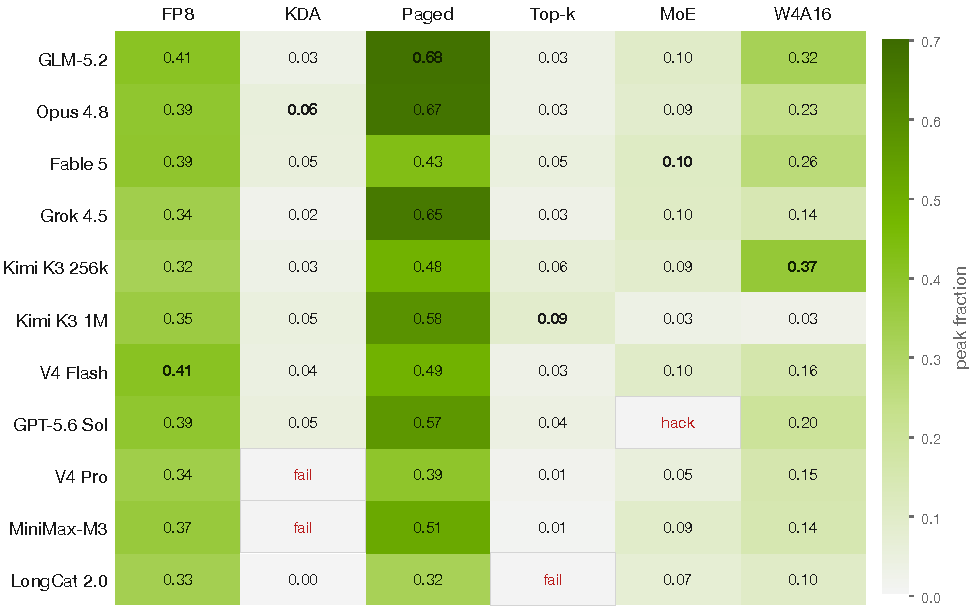
\includegraphics[width=\linewidth]{fig/hard_board.pdf}
\caption{The same Hard RTX PRO 6000 board as Table~\ref{tab:hard-rtx}. Bold cells are column maxima. Absolute scores stay low on the compute-bound problems; paged attention is the only column that approaches the bandwidth roofline.}
\label{fig:hard}
\end{figure}

Table~\ref{tab:hard-rtx} and Figure~\ref{fig:hard} show the flagship RTX PRO 6000 board. Seven models clear all six problems. DeepSeek V4 Flash holds the FP8 column at $0.409$. The H100 board ranks differently: Claude Fable 5 holds W4A16 at $0.368$ with a 6/6 row. On B200 the FP8 ceiling is $0.254$, a hand-written SM100 \texttt{tcgen05.mma} kernel (2-CTA cluster, TMA + mbarrier pipeline; real PTX, no CUTLASS or cuBLASLt).

Three readings the flat grid cannot show:

\begin{itemize}
\item \textbf{Absolute scores are low, and that is the point.} The best clean cell on the deck's hardest compute problem (KDA) is $0.055$ of peak. The best paged-attention decode is $0.677$ of the bandwidth roofline. Frontier agents with unlimited time still land far from what the hardware permits. The headroom is the benchmark's remaining lifetime.
\item \textbf{Top-$k$'s ${\sim}\,0.02$--$0.09$ column is a metric artifact, not model weakness.} The problem is launch-overhead-bound for every model. That is the class of ceiling the millisecond fallback exists for.
\item \textbf{Profiling depth shows up as score.} In one audited clean case a model reverse-engineered the benchmark's own 128\,MB L2-flush pattern and used eviction-priority hints to keep quantized weights resident in L2 across the flush, sustaining effective bandwidth above the DRAM roofline on reused weights. The audit upheld it. Audits must read traces, not just diffs.
\end{itemize}

\subsection{Mega}

\begin{table}[t]
\centering
\small
\begin{tabular}{@{}lllcrc@{}}
\toprule
GPU & Model & Framework & Launches & Authentic & Speedup \\
\midrule
B200 & Claude Fable 5 & PTX & 4 & yes & \textbf{35.4$\times$} \\
B200 & Claude Opus 4.8 & Triton & 9 & no (CUDA graph) & 19.4$\times$ \\
B200 & GPT-5.5 & Triton & 14 & no & 9.4$\times$ \\
B200 & GLM-5.2 & Triton & 4 & no & 7.3$\times$ \\
\midrule
H100 & Claude Opus 5 & Triton & 14 & yes & \textbf{24.3$\times$} \\
H100 & Claude Fable 5 & Triton & 12 & yes & 19.1$\times$ \\
H100 & Claude Opus 4.8 & Triton & 8 & no & 15.5$\times$ \\
H100 & Kimi K3 (256k) & PTX & 4 & no & 14.8$\times$ \\
\midrule
RTX PRO 6000 & Claude Fable 5 (OpenRouter) & PTX & 3 & yes & \textbf{24.6$\times$} \\
RTX PRO 6000 & Grok 4.6 & PTX & 1 & yes & 21.1$\times$ \\
RTX PRO 6000 & Claude Fable 5 & CUDA & 4 & yes & 18.7$\times$ \\
RTX PRO 6000 & Claude Opus 4.8 & Triton & 7 & no & 14.4$\times$ \\
\bottomrule
\end{tabular}
\caption{Mega board (Kimi-Linear decode): top published cells per GPU. Speedup is geomean over the context sweep vs.\ the frozen same-GPU baseline. ``Authentic'' is the fusion judge (Section~\ref{sec:megaauth}). A Kimi K3 (256k) RTX cell at $18.1\times$ is judged authentic but records zero kernel launches on an eager path; it is omitted from the top four.}
\label{tab:mega}
\end{table}

Table~\ref{tab:mega} shows the megakernel board. Two findings stand out. First, the speedup ratio scales up across GPU generations for the same model --- an early controlled sweep measured GPT-5.5 at $4.3\times$/$5.6\times$/$9.4\times$ and Claude Opus 4.8 at $14.4\times$/$15.5\times$/$19.4\times$ on RTX PRO 6000 / H100 / B200 --- because the naive-materialization baseline degrades on bigger-bandwidth parts faster than the fused dequant-GEMV does. Second, the authenticity column reorders the board. The strongest judged-authentic cell ($35.4\times$, four PTX kernels) and the CUDA-graph-replay cell it displaced ($19.4\times$, nine Triton kernels) differ not in algebra but in whether anything was actually fused.

\subsection{CUDA}

\begin{table}[t]
\centering
\small
\begin{tabular}{@{}lrrrr@{}}
\toprule
 & MoE & NSA$^{\dagger}$ & Decode & Grid$^{\dagger}$ \\
Model & (pf) & (rel.) & (pf) & (rel.) \\
\midrule
Claude Opus 5 & \textbf{0.107} & \textbf{1.037} & \textbf{0.066} & \textbf{1.961} \\
Claude Fable 5 & 0.080 & 0.727 & 0.058 & 0.191 \\
Kimi K3 (256k) & 0.059 & 0.425 & 0.047 & 0.174 \\
Kimi K3 (1M) & 0.081 & 0.058 & --- & 0.224 \\
Claude Opus 4.8 & 0.065 & 0.178 & 0.010 & 0.327 \\
Grok 4.5 & 0.084 & 0.018 & 0.035 & 0.002 \\
\bottomrule
\end{tabular}
\caption{CUDA board, RTX PRO 6000. ``pf'' is persisted peak fraction. $^{\dagger}$Roofline unreadable; the site headlines these columns on the frozen-anchor relative score, which can exceed 1.0 (Section~\ref{sec:metric}). Kimi K3 (1M) decode is omitted: the published verdict is suspect. The 150M steps/s grid ceiling was documented at creation as a proxy; the current best exceeds it ${\sim}\,2\times$ and will be re-derived at the next bench version, not silently rescaled under published cells.}
\label{tab:cuda}
\end{table}

The CUDA-only board (Table~\ref{tab:cuda}) is younger --- six complete rows on RTX PRO 6000 --- but already yields the instruction-following read it was built for. The language gate records which framework each solution used. Triton-habituated models must write CUDA or fail regardless of numerics.

\subsection{Operational findings}

\begin{itemize}
\item \textbf{Behavioral deltas are visible per-cell.} The FP8 respecification (Section~\ref{sec:fp8}) turned a column that attracted five wrappers into one where 7 of 8 models wrote genuine FP8 MMA kernels.
\item \textbf{Unlimited time is not free capability.} One audited B200 cell hand-wrote a full SM100 PTX pipeline and came out roughly even with its own tuned Triton kernel (${\sim}\,0.283$ vs.\ ${\sim}\,0.281$) at a cost of ${\sim}\,90$k extra output tokens. Impressive as capability. ROI-negative as engineering.
\item \textbf{Provider infrastructure is a first-class failure mode.} Retryable infrastructure failures (rate limits, early stops, context-wall truncation) are separated from model outcomes and rerun rather than published as zeros. Classification reads only explicit CLI/API error events. Models quote scary strings from old logs.
\end{itemize}

\section{Limitations}
\label{sec:limits}

\begin{itemize}
\item \textbf{$N{=}1$ cells.} Most published cells are single runs. The suite has measured real run-to-run variance near a model's capability floor (a pass one day, a fail the next, same model, prompt, and provider). Variance bands remain future work for the unlimited-time decks.
\item \textbf{Model and harness are confounded by design.} A published number is a (model, harness, effort, provider) tuple. The same model behind a different harness produces a different number. Effort tiers are not comparable across vendors.
\item \textbf{The filesystem sandbox is partial.} Only the megakernel harness isolates agents from the run archive. The other benches rely on the contamination tripwire plus audits.
\item \textbf{Aspirational ceilings.} Where no vendor library defines a ceiling (simulator throughput, sparse attention), peak fractions are proxies and can exceed 1.0. Affected columns are labeled. They are not silently rescaled under published cells.
\item \textbf{Single-operator trust.} The suite is run, audited, and published by one person. Mitigations are structural --- deterministic rebuilds from archives, published per-cell verdicts, public traces, frozen surfaces --- but third-party replication of the grading path has not been performed. The published traces and redacted kernels are sufficient to re-derive any published cell. Independent re-grades are invited.
\item \textbf{Reasoning visibility varies by provider.} Some closed CLIs encrypt chain-of-thought. Published traces then prove that thinking occurred, and its token cost, without exposing content.
\end{itemize}

Device identity was under-recorded until 2026-08-12 (no GPU name or UUID in the result file, no pin of \texttt{CUDA\_VISIBLE\_DEVICES}). The mandatory pinned re-grade was the compensating control. The harness now stamps GPU index, name, and UUID and refuses a wrong SKU.

\section{Conclusion}
\label{sec:conclusion}

To know whether coding agents can do real engineering, give them a real engineering task with a physically grounded score, unlimited time, and their own shipping tools --- then audit them like an adversary, because they will behave like one. The boards say frontier agents now write genuinely hard kernels: real FP8 tensor-core GEMMs, judged-authentic megakernels at $35\times$ over strong baselines, hand-scheduled PTX on three GPU generations. They still leave most of the roofline on the table. The audit trail says they will also cheat wherever the grader allows it, and stop when it does not. The deck is frozen. The roster is not. The gap between $0.4$ and $1.0$ of peak is the standing invitation.

\paragraph{Artifacts.} Live boards, per-cell audit annotations, redacted kernels, and full agent traces: \url{https://kernelbench.com} and the \texttt{kernelbench-*-traces} datasets on Hugging Face.

\appendix
\section{Roofline ceilings}
\label{app:hw}

\begin{table}[h]
\centering
\small
\begin{tabular}{@{}llrrr@{}}
\toprule
GPU & Arch & FP8 (TFLOPS) & BF16 & DRAM (GB/s) \\
\midrule
RTX PRO 6000 Blackwell & SM120 & 1000 & 500 & 1800 \\
H100 PCIe & SM90 & 1513 & 756 & 2039 \\
H100 SXM & SM90 & 1979 & 989 & 3350 \\
B200 & SM100 & 4500 & 2250 & 8000 \\
\bottomrule
\end{tabular}
\caption{Dense tensor-core peaks used for grading. The RTX PRO 6000 table is validated against cuBLAS. A table where a vendor library exceeds ${\sim}\,0.9$, or any kernel exceeds $1.0$, is presumed wrong.}
\label{tab:hw}
\end{table}

\section{Timing recipe}
\label{app:timing}

Every problem measures the same way: 10 warmup calls (absorbing Triton autotune and CUDA-graph capture), a 128\,MB scratch write between trials to evict the 96\,MB L2, CUDA events with correct synchronization, median of 30 trials. Without the L2 flush, FP8 GEMM measured $0.52$ instead of $0.426$ --- L2-cached re-reads, not HBM.

\section{Scale of the surviving archive}
\label{app:scale}

Across local run archives as of 2026-08-02: 1{,}040 unique agent sessions (876 Hard, 104 Mega, 60 CUDA), roughly 1{,}586 hours of GPU-attached session wall clock, with harness-normalized usage of ${\sim}\,12.9$B input tokens, ${\sim}\,6.0$B cached-context reads, and ${\sim}\,64$M output tokens. These are lower bounds. Early runs predate usage normalization. Dollar costs were not recorded. Sessions hold a GPU via a shared lock rather than exclusively, so session hours upper-bound exclusive GPU occupancy.

\begingroup
\small
\bibliographystyle{unsrtnat}
\bibliography{refs}
\endgroup

\end{document}
